%Texlive-full Version 3.141592-1.40.3 (Web2C 7.5.6)
%Kile Version 2.0.83
%File associated : SoFa_Logo.ps , FF.ps

\documentclass[a4paper,10pt]{article}
\usepackage[utf8x]{inputenc}
\usepackage[T1]{fontenc} 

\usepackage{lmodern}
\usepackage[a4paper]{geometry}
%\usepackage[frenchb]{babel}
\usepackage{graphicx}
\usepackage{hyperref}

\usepackage{pstricks}
\usepackage{pst-node}
%\usepackage{wrapfig}
\usepackage{amsmath}
\usepackage{amsfonts}
\usepackage{amssymb}
\usepackage{textcomp}
%\usepackage{mathaccent}
\usepackage{listings}
\lstset{language=C++,basicstyle=\scriptsize \color{green},identifierstyle=\color{orange},keywordstyle=[1]\color{blue},columns=fullflexible,commentstyle=\textit}

\usepackage{color}



\begin{document}
%%%%%%%%%%%%%%%%%%   LOGO  %%%%%%%%%%%%%%%%%%%%%%%%%
\begin{center}
\rput(6,1.5){\href{http://www.sofa-framework.org/}{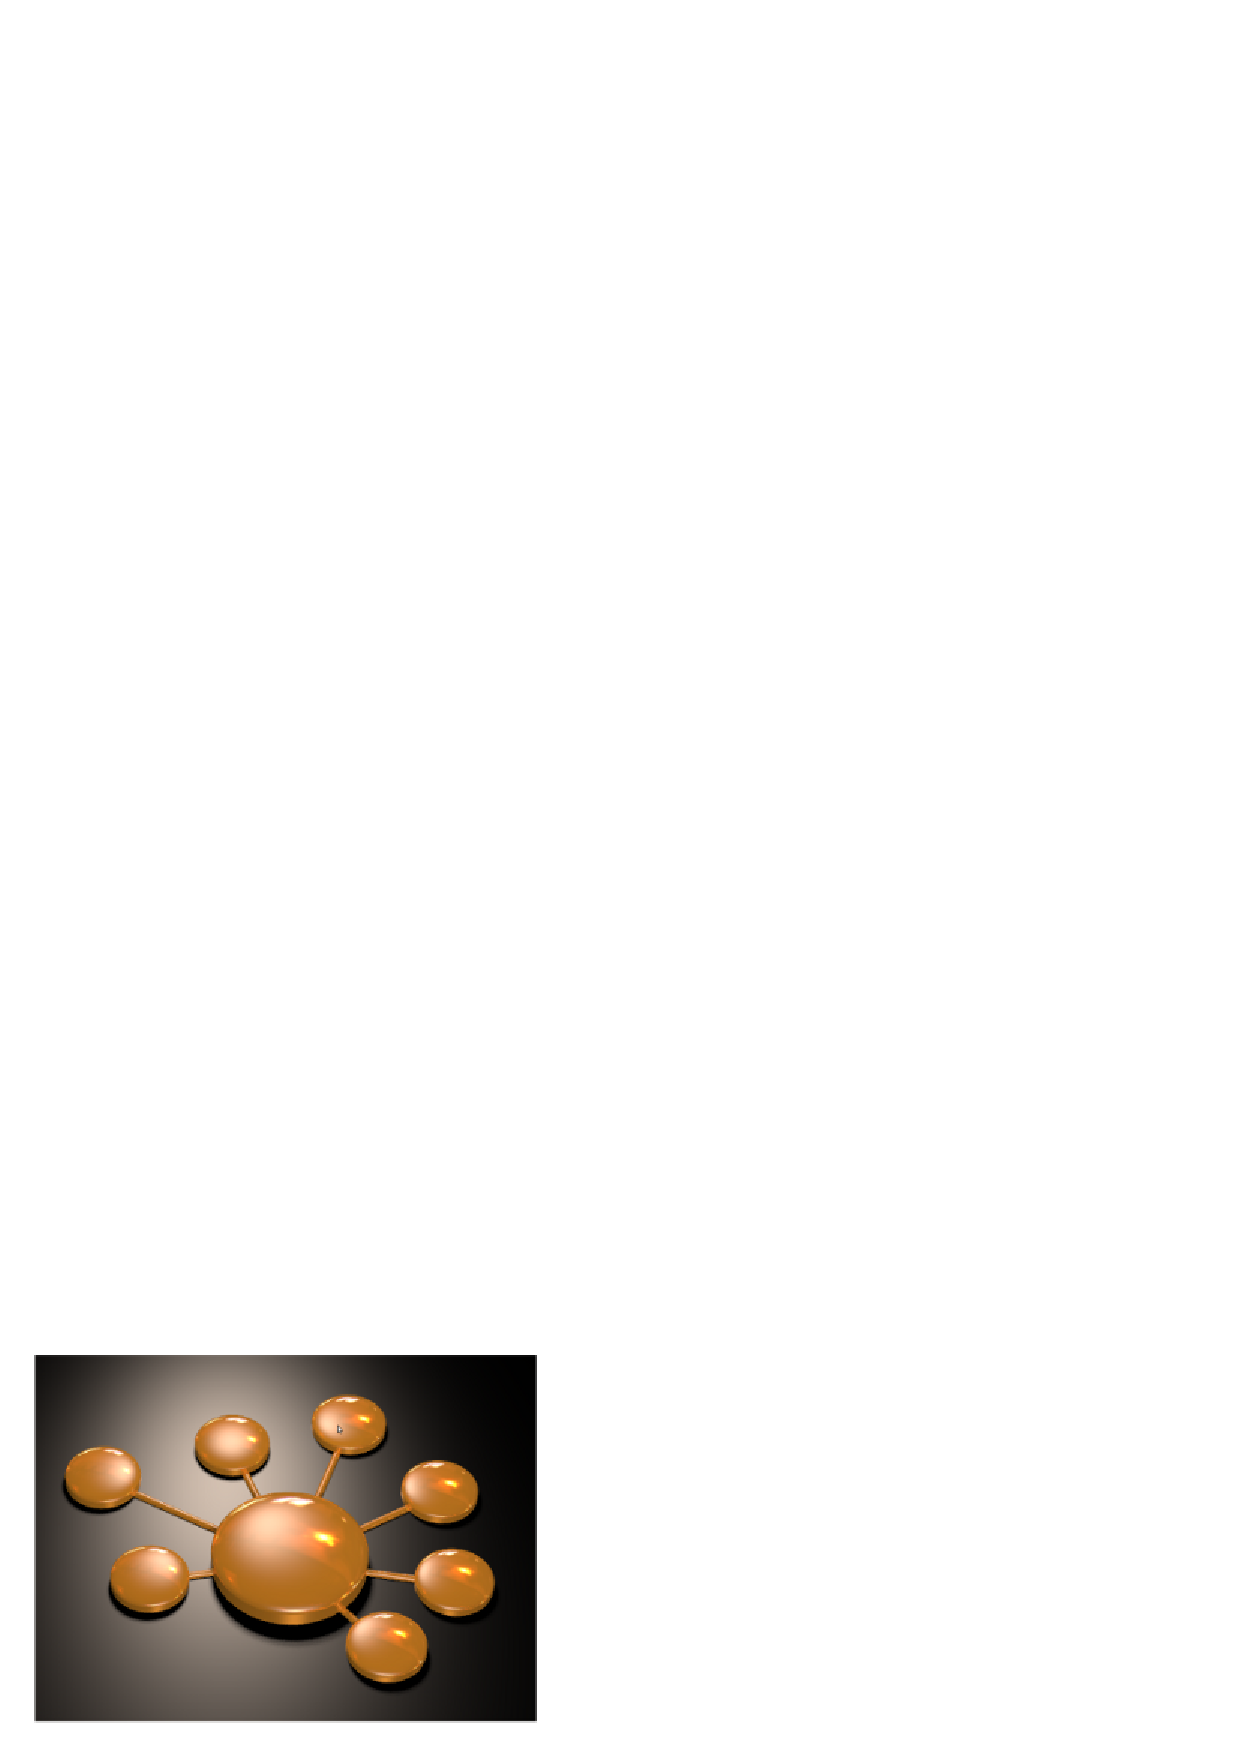
\includegraphics[scale=0.3]{SoFa_Logo}}}
\rput(-4,1.5){\href{http://www.sofa-framework.org/}{
		\begin{tabular}{l}
		\resizebox{4cm}{0.6cm}{SOFA} \\ 
		\resizebox{6cm}{0.3cm}{Simulation Open Framework Architecture}
		\end{tabular}
		}
	    }
\end{center}
%%%%%%%%%%%%%%%%%%   LOGO  %%%%%%%%%%%%%%%%%%%%%%%%%

%%%%%%%%%%%%%%%%%% DOCUMENT TITLE %%%%%%%%%%%%%%%%%%%%%%%%% To be deleted when include in the global document
%\chapter{Mapping} %\section{Rigid Mapping} 
\vspace{1.5cm}
\begin{center}\resizebox{7cm}{0.6cm}{Linear Solver}\end{center}
%%%%%%%%%%%%%%%%%% DOCUMENT TITLE %%%%%%%%%%%%%%%%%%%%%%%%%

%%%%%%%%%%%%%%%%%%%%%%%%%%%%%%%%%%%%%%%%%%%%%%%%%%%%%%%%%%%%%%%%%%%%%%%%%%%%%%%%%%%%%%%%%
%=======================================================================================%
%%%%%%%%%%%%%%%%%%%%%%%%%%%%%%%%%%%%%%%%%%%%%%%%%%%%%%%%%%%%%%%%%%%%%%%%%%%%%%%%%%%%%%%%%
%\section{Linear Solver}% for adding to the global document of SOFA

\section{Linear Solver}
\paragraph{Abstract : }
%%%%%%%%%%%%%%%%%%   LOGO  %%%%%%%%%%%%%%%%%%%%%%%%%
%%%%%%%%%%%%%%%%%%   LOGO  %%%%%%%%%%%%%%%%%%%%%%%%%
introducing the simulation scene graph where there are mapped ms, mapping, interaction forcefield between real DOF and mapped MS

\subsection{Direct Solvers }
Present here the matrix structure in the generale case, where there are several mapped mechanical states and interactions between them. Explain the structure : principale blocs, diagonal bloc (self-stiffness), non-diagonal blocs (interaction-stiffness), mapping blocs J can be seen as a bloc ...
\subsection{Context in SOFA }
Identifying the problem in SOFA where there are a scene but not all nodes has stiffness, or not all mapping has matrix J

//           case1                                           case2
//      |               |                                  |       |
//     MS1             MS2                                MS1     MS2
//      |               |                                 /      /
//     mapA            mapB                             map   Inter
//      |               |                                 \   /
//     MS3 ---Inter--  MS4                                MS3/
//
//    K11 += JAt * K33 * JA                         K11 += Jt * K33 * J
//    K22 += JBt * K44 * JB                         K12 += Jt * I32
//    K12 += JAt * I34 * JB                         K21 +=      I32 * J
//    K21 += JBt * I43 * JA
\subsubsection{self-stiffness propagation }
\[
 K_{11} += J^t * K_{22} * J
\]
\subsubsection{interaction-stiffness propagation }
\paragraph{Interaction beweent Real Mechanical Object and Mapped Mechanical Object}
\begin{center}
  \includegraphics[scale=0.3]{interaction_Real_Mapped}
\end{center}
\[
K_{11} += J^t * K_{33} * J 
\]
\[
K_{12} += J^t * I_{32}
\]
\[
K_{21} += I_{32} * J 
\]
\paragraph{Interaction beweent Mapped Mechanical Object and Mapped Mechanical Object}
\begin{center}
  \includegraphics[scale=0.3]{interaction_Mapped_Mapped}
\end{center}
\[
K_{11} += JA^t * K_{33} * JA 
\]
\[
K_{22} += JB^t * K_{44} * JB 
\]
\[
K_{12} += JA^t * I_{34} * JB 
\]
\[
K_{21} += JB^t * I_{43} * JA 
\]
\subsection{Iterative Solvers }
\subsection{Preconditioner }



						      %%%%%%%%%%%%%%%%%%%%%%%%%%  Writer %%%%%%%%%%%%%%%%%%%%%%%%
						      \begin{flushright}
						      Document written by \\
						      \href{mailto:chi-thanh.nguyen@inria.fr}{{\textbf {Chi Thanh NGUYEN}}} \\
						      INRIA Lille
						      \end{flushright}
						      %%%%%%%%%%%%%%%%%%%%%%%%%%  Writer %%%%%%%%%%%%%%%%%%%%%%%%

%\bibliographystyle{siam}
%\bibliography{mybiblio}
\end{document}
